%%%%%%%%%%%%%%%%%%%%%%%%%%%%%%%%%%%%%%%%%
% Beamer Presentation
% LaTeX Template
% Version 1.0 (10/11/12)
%
% This template has been downloaded from:
% http://www.LaTeXTemplates.com
%
% License:
% CC BY-NC-SA 3.0 (http://creativecommons.org/licenses/by-nc-sa/3.0/)
%
%%%%%%%%%%%%%%%%%%%%%%%%%%%%%%%%%%%%%%%%%

%----------------------------------------------------------------------------------------
%	PACKAGES AND THEMES
%----------------------------------------------------------------------------------------

\documentclass[handout]{beamer}

\mode<presentation> {

% The Beamer class comes with a number of default slide themes
% which change the colors and layouts of slides. Below this is a list
% of all the themes, uncomment each in turn to see what they look like.

%\usetheme{default}
%\usetheme{AnnArbor}
%\usetheme{Antibes}
%\usetheme{Bergen}
%\usetheme{Berkeley}
%\usetheme{Berlin}
%\usetheme{Boadilla}
%\usetheme{CambridgeUS}
%\usetheme{Copenhagen}
%\usetheme{Darmstadt}
%\usetheme{Dresden}
%\usetheme{Frankfurt}
%\usetheme{Goettingen}
%\usetheme{Hannover}
%\usetheme{Ilmenau}
%\usetheme{JuanLesPins}
%\usetheme{Luebeck}
\usetheme{Madrid}
%\usetheme{Malmoe}
%\usetheme{Marburg}
%\usetheme{Montpellier}
%\usetheme{PaloAlto}
%\usetheme{Pittsburgh}
%\usetheme{Rochester}
%\usetheme{Singapore}
%\usetheme{Szeged}
%\usetheme{Warsaw}

% As well as themes, the Beamer class has a number of color themes
% for any slide theme. Uncomment each of these in turn to see how it
% changes the colors of your current slide theme.

%\usecolortheme{albatross}
%\usecolortheme{beaver}
%\usecolortheme{beetle}
%\usecolortheme{crane}
%\usecolortheme{dolphin}
%\usecolortheme{dove}
%\usecolortheme{fly}
%\usecolortheme{lily}
%\usecolortheme{orchid}
%\usecolortheme{rose}
%\usecolortheme{seagull}
%\usecolortheme{seahorse}
%\usecolortheme{whale}
%\usecolortheme{wolverine}

%\setbeamertemplate{footline} % To remove the footer line in all slides uncomment this line
%\setbeamertemplate{footline}[page number] % To replace the footer line in all slides with a simple slide count uncomment this line

%\setbeamertemplate{navigation symbols}{} % To remove the navigation symbols from the bottom of all slides uncomment this line
}

\usepackage{graphicx} % Allows including images
\usepackage{booktabs} % Allows the use of \toprule, \midrule and \bottomrule in tables
\usepackage{cool}
\usepackage{tikz}
\usepackage{amsmath}
\DeclareMathOperator*{\argmax}{argmax}
\DeclareMathOperator*{\argmin}{argmin}
\usetikzlibrary{positioning}

%----------------------------------------------------------------------------------------
%	TITLE PAGE
%----------------------------------------------------------------------------------------


\title[Derivatives Chapter]{A Guided Tour of \href{http://stanford.edu/~ashlearn/RLForFinanceBook/book.pdf}{\underline{\textcolor{yellow}{Chapter 7}}}: \\  Derivatives Pricing and Hedging} 

\author{Ashwin Rao} % Your name
\institute[Stanford] % Your institution as it will appear on the bottom of every slide, may be shorthand to save space
{
ICME, Stanford University
 % Your institution for the title page
}

\date{\today} % Date, can be changed to a custom date

\begin{document}
\begin{frame}
\titlepage % Print the title page as the first slide
\end{frame}



\begin{frame}
\frametitle{Brief Overview of Derivatives}
\begin{itemize}[<+->]
\item Term {\em Derivative} comes from the word {\em Derived}
\item Financial product whose structure (and hence, {\em value}) is derived from the {\em performance} of an {\em underlying} entity
\item Technically a legal contract between buyer and seller that is either:
\begin{itemize}[<+->]
\item {\em Lock-type}: {\em Entitles} buyer to future contingent-cashflow ({\em payoff})
\item {\em Option-type:} Buyer has future {\em choices}, leading to contingent-cashflow
\end{itemize}
\item Some common derivatives:
\begin{itemize}[<+->]
\item Forward  - Contract to deliver/receive asset on future date for fixed cash
$$\text{Forward Payoff: } f(X_t) = X_t - K$$
\item European Option - {\em Right} to buy/sell on future data at agreed price
$$\text{Call and Put Option Payoff: } \max(X_t - K, 0) \text{ and} \max(K - X_t, 0)$$
\item American Option - Can exercise option on {\em any day} before expiration
\end{itemize}
\item Why do we need derivatives?
\begin{itemize}[<+->]
\item To protect against adverse market movements ({\em risk-management})
\item To express a market view {\em cheaply} (leveraged trade)
\end{itemize}
\end{itemize}
\end{frame}

\begin{frame}
\frametitle{Derivatives Pricing and Hedging problems as MDPs}
\pause
\begin{itemize}[<+->]
\item {\em Pricing}: Determination of fair value of an asset or derivative
\item {\em Hedging}: Protect against market movements with ``opposite'' trades
\item {\em Replication}: Clone payoff of a derivative with trades in other assets
\item We consider two applications of Stochastic Control here:
\begin{itemize}[<+->]
\item Optimal Exercise of American Options in an idealized setting
\item Optimal Hedging of Derivatives Portfolio in a real-world setting
\end{itemize}
\item Both problems enable us to price the respective derivatives
\item Expressing these problems as MDP Control brings ADP/RL into play
\item Optimal Exercise of American Options is Optimal Stopping problem
\item So we start by learning about Stopping Time and Optimal Stopping
\end{itemize}
\end{frame}

\begin{frame}
\frametitle{Stopping Time}
\pause
\begin{itemize}[<+->]
\item Stopping time $\tau$ is a ``random time'' (random variable) interpreted as time at which a given stochastic process exhibits certain behavior
\item Stopping time often defined by a ``stopping policy'' to decide whether to continue/stop a process based on present position and past events
\item Random variable $\tau$ such that $Pr[\tau \leq t]$ is in $\sigma$-algebra $\mathcal{F}_t$, for all $t$
\item Deciding whether $\tau \leq t$ only depends on information up to time $t$
\item Hitting time of a Borel set $A$ for a process $X_t$ is the first time $X_t$ takes a value within the set $A$
\item Hitting time is an example of stopping time. Formally, 
$$T_{X,A} = \min \{t \in \mathbb{R} | X_t \in A\}$$
eg: Hitting time of a process to exceed a certain fixed level
\end{itemize}
\end{frame}

\begin{frame}
\frametitle{Optimal Stopping Problem}
\pause
\begin{itemize}[<+->]
\item Optimal Stopping problem for Stochastic Process $X_t$: 
$$W(x) = \max_{\tau} \mathbb{E}[H(X_{\tau})|X_0 = x]$$
 where $\tau$ is a set of stopping times of $X_t$, $W(\cdot)$ is called the Value function, and $H$ is the Reward function.
\item Note that sometimes we can have several stopping times that maximize $\mathbb{E}[H(X_{\tau})]$ and we say that the optimal stopping time
is the smallest stopping time achieving the maximum value.
\item Example of Optimal Stopping: Optimal Exercise of American Options
\begin{itemize}
\item $X_t$ is risk-neutral process for underlying security's price
\item $x$ is underlying security's current price
\item $\tau$ is set of exercise times corresponding to various stopping policies
\item $W(\cdot)$ is American option price as function of underlying's current price
\item $H(\cdot)$ is the option payoff function, adjusted for time-discounting
\end{itemize}
\end{itemize}
\end{frame}


\begin{frame}
\frametitle{Optimal Stopping Problems as Markov Decision Processes}
\pause
\begin{itemize}[<+->]
\item We formulate Stopping Time problems as Markov Decision Processes
\item {\em State} is $X_t$
\item {\em Action} is Boolean: Stop or Continue
\item {\em Reward} always 0, except upon Stopping (when it is $=H(X_{\tau})$)
\item {\em State}-transitions governed by the Stochastic Process $X_t$
\item For discrete time steps, the Bellman Optimality Equation is:
$$V^*(X_t) = \max(H(X_t), \mathbb{E}[V^*(X_{t+1})|X_t])$$
\item For finite number of time steps, we can do a simple backward induction algorithm from final time step back to time step 0
\end{itemize}
\end{frame}


\begin{frame}
\frametitle{Mainstream approaches to American Option Pricing}
\pause
\begin{itemize}[<+->]
\item American Option Pricing is Optimal Stopping, and hence an MDP
\item So can be tackled with Dynamic Programming or RL algorithms
\item But let us first review the mainstream approaches
\item For some American options, just price the European, eg: vanilla call
\item When payoff is not path-dependent and state dimension is not large, we can do backward induction on a binomial/trinomial tree/grid
\item Otherwise, the standard approach is \href{https://people.math.ethz.ch/~hjfurrer/teaching/LongstaffSchwartzAmericanOptionsLeastSquareMonteCarlo.pdf}{\underline{\textcolor{blue}{Longstaff-Schwartz algorithm}}}
\item Longstaff-Schwartz algorithm combines 3 ideas:
\begin{itemize}
\item Valuation based on Monte-Carlo simulation
\item Function approximation of continuation value for in-the-money states
\item Backward-recursive determination of early exercise states
\end{itemize}
\item RL is an attractive alternative to Longstaff-Schwartz algorithm
\end{itemize}
\end{frame}

\begin{frame}
\frametitle{Binomial Tree for Backward Induction}
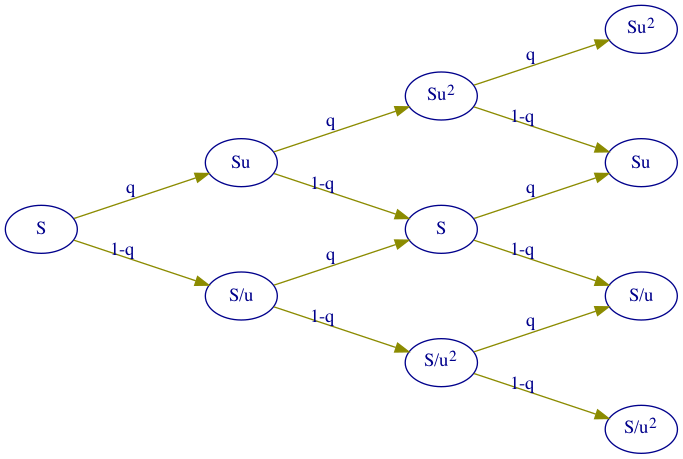
\includegraphics[scale=0.4]{binomial_tree.png}
\end{frame}

\begin{frame}
\frametitle{Optimal Exercise Boundary of American Put Option}
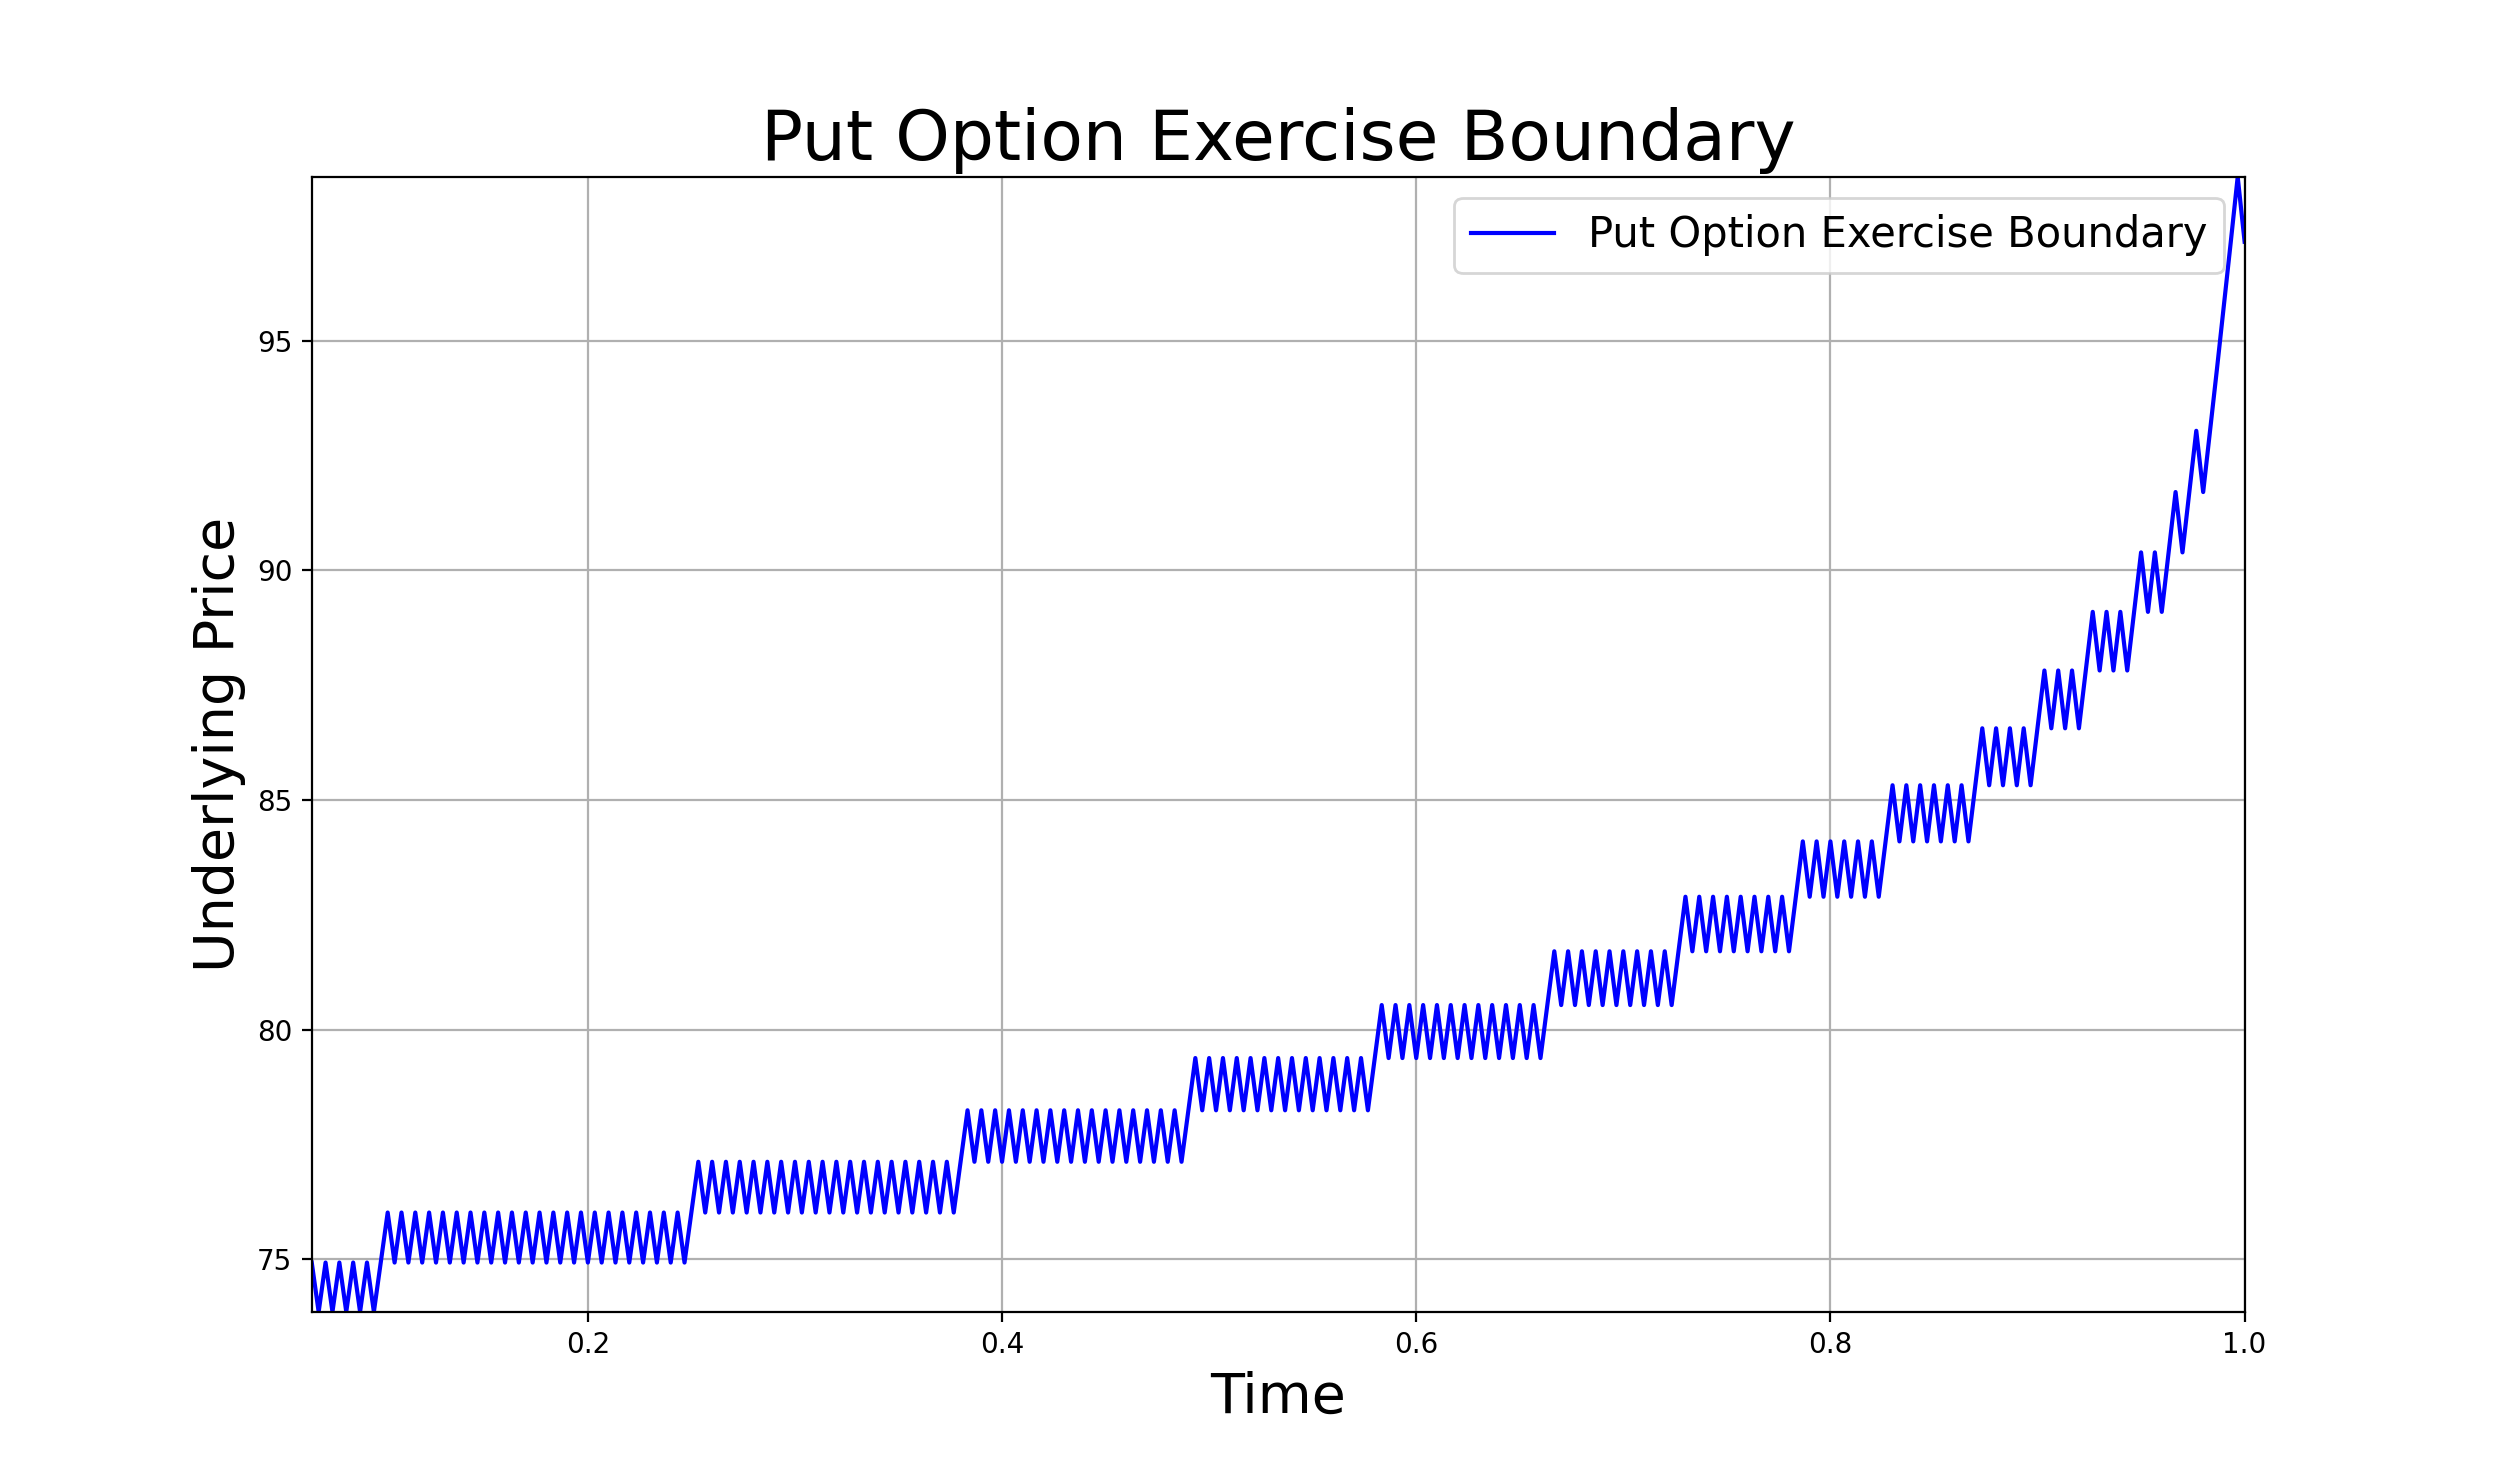
\includegraphics[scale=0.4]{put_option_ex_boundary.png}
\end{frame}

\begin{frame}
\frametitle{Classical Pricing and Hedging of Derivatives}
\pause
\begin{itemize}[<+->]
\item Classical Pricing/Hedging Theory is based on a few core concepts:
\begin{itemize}
\item {\bf Arbitrage-Free Market} - where you cannot make money from nothing
\item {\bf Replication} - when the payoff of a {\em Derivative} can be constructed by assembling (and rebalancing) a portfolio of the underlying securities
\item {\bf Complete Market} - where payoffs of all derivatives can be replicated
\item {\bf Risk-Neutral Measure} - Altered probability measure for movements of underlying securities for mathematical convenience in pricing
\end{itemize}

\item Assumptions of \href{https://github.com/coverdrive/technical-documents/blob/master/finance/ArbitrageCompleteness.pdf}{\underline{\textcolor{blue}{arbitrage-free and completeness}}}
lead to (dynamic, exact, unique) replication of derivatives with the underlying securities
\item Assumptions of frictionless trading provide these idealistic conditions
\item Frictionless := continuous trading, any volume, no transaction costs
\item Replication strategy gives us the pricing and hedging solutions
\item This is the foundation of the famous Black-Scholes formulas
\item However, the real-world has many frictions $\Rightarrow$ {\em Incomplete Market}
\item ... where derivatives cannot be exactly replicated
\end{itemize}
\end{frame}

\begin{frame}
\frametitle{Pricing and Hedging in an Incomplete Market}
\pause
\begin{itemize}[<+->]
\item In an incomplete market, we have multiple risk-neutral measures
\item So, multiple derivative prices (each consistent with no-arbitrage)
\item The market/trader ``chooses'' a risk-neutral measure (hence, price)
\item This ``choice'' is typically made in ad-hoc and inconsistent ways
\item Alternative approach is for a trader to play {\em Portfolio Optimization}
\item Maximizing ``risk-adjusted return'' of the derivative plus hedges
\item Based on a specified preference for trading risk versus return
\item This preference is equivalent to specifying a \href{https://github.com/coverdrive/technical-documents/blob/master/finance/cme241/UtilityTheoryForRisk.pdf}{\underline{\textcolor{blue}{Utility function}}}
\item Reminiscent of the Portfolio Optimization problem we've seen before
\item Likewise, we can set this up as a stochastic control (MDP) problem
\item Where the decision at each time step is: {\em Trades in the hedges}
\item So what's the best way to solve this MDP?
\end{itemize}
\end{frame}


\begin{frame}
\frametitle{Deep Reinforcement Learning (DRL)}
\pause
\begin{itemize}[<+->]
\item Dynamic Programming not suitable in practice due to:
\begin{itemize}
\item Curse of Dimensionality
\item Curse of Modeling
\end{itemize}
\item So we solve the MDP with {\em Deep Reinforcement Learning} (DRL)
\item The idea is to use real market data and real market frictions
\item Developing realistic simulations to derive the optimal policy
\item The optimal policy gives us the (practical) hedging strategy
\item The optimal value function gives us the price (valuation)
\item Formulation based on \href{https://papers.ssrn.com/sol3/papers.cfm?abstract_id=3355706}{\underline{\textcolor{blue}{Deep Hedging paper}}} by J.P.Morgan researchers
\item More details in the \href{https://papers.ssrn.com/sol3/papers.cfm?abstract_id=3355706}{\underline{\textcolor{blue}{prior paper}}} by some of the same authors
\end{itemize}
\end{frame}

\begin{frame}
\frametitle{Problem Setup}
\pause
\begin{itemize}[<+->]
\item We will simplify the problem setup a bit for ease of exposition
\item This model works for more complex, more frictionful markets too
\item Assume time is in discrete (finite) steps $t = 0, 1, \ldots, T$
\item Assume we have a position (portfolio) $D$ in $m$ derivatives
\item Assume each of these $m$ derivatives expires in time $ \leq T$
\item Portfolio-aggregated {\em Contingent Cashflows} at time $t$ denoted $X_t \in \mathbb{R}$
\item Assume we have $n$ underlying market securities as potential hedges
\item Hedge positions (units held) at time $t$ denoted $\alpha_t \in \mathbb{R}^n$
\item Cashflows per unit of hedges held at time $t$ denoted $Y_t \in \mathbb{R}^n$
\item Prices per unit of hedges at time $t$ denoted $P_t \in \mathbb{R}^n$
\item PnL position at time $t$ is denoted as $\beta_t \in \mathbb{R}$
\end{itemize}
\end{frame}

\begin{frame}
\frametitle{States and Actions}
\pause
\begin{itemize}[<+->]
\item Denote state space at time $t$ as $\mathcal{S}_t$, state at time $t$ as $s_t \in \mathcal{S}_t$
\item Among other things, $s_t$ contains $t, \alpha_t, P_t, \beta_t, D$
\item $s_t$ will include any market information relevant to trading actions
\item For simplicity, we assume $s_t$ is just the tuple $(t, \alpha_t, P_t, \beta_t, D)$
\item Denote action space at time $t$ as $\mathcal{A}_t$, action at time $t$ as $a_t \in \mathcal{A}_t$
\item $a_t$ represents units of hedges traded (positive for buy, negative for sell)
\item Trading restrictions (eg: no short-selling) define $\mathcal{A}_t$ as a function of $s_t$
\item State transitions $P_{t+1}|P_t$ available from a {\em simulator}, whose internals are estimated from real market data and realistic assumptions
\end{itemize}
\end{frame}

\begin{frame}
\frametitle{Sequence of events at each time step $t=0, \ldots, T$}
\pause
\begin{enumerate}[<+->]
\item Observe state $s_t = (t, \alpha_t, P_t, \beta_t, D)$
\item Perform action (trades) $a_t$ to produce trading PnL $= - a_t \cdot P_t$
\item Trading transaction costs, example $= - \gamma P_t \cdot |a_t|$ for some $\gamma > 0$
\item Update $\alpha_t$ as: $\alpha_{t+1} = \alpha_t + a_t$ \\(force-liquidation at termination means $a_T= -\alpha_T$)
\item Realize cashflows (from updated positions) $=X_{t+1} + \alpha_{t+1} \cdot Y_{t+1}$
\item Update PnL $\beta_t$ as:
$$\beta_{t+1} = \beta_t - a_t \cdot P_t - \gamma P_t \cdot |a_t|  + X_{t+1} + \alpha_{t+1} \cdot Y_{t+1}$$
\item Reward $r_t = 0$ for all $t = 0, \ldots, T-1$ and $r_T = U(\beta_{T+1})$ for an appropriate concave Utility function $U$ (based on risk-aversion)
\item Simulator evolves hedge prices from $P_t$ to $P_{t+1}$
\end{enumerate}
\end{frame}

\begin{frame}
\frametitle{Pricing and Hedging}
\pause
\begin{itemize}[<+->]
\item Assume we now want to enter into an incremental position (portfolio) $D'$ in $m'$ derivatives (denote the combined position as $D \cup D'$)
\item We want to determine the {\em Price} of the incremental position $D'$, as well as the hedging strategy for $D'$
\item Denote the Optimal Value Function at time $t$ as $V_t^* : \mathcal{S}_t \rightarrow \mathbb{R}$
\item Pricing of $D'$ is based on the principle that introducing the incremental position of $D'$ together with a calibrated cashflow (Price) at $t=0$ should leave the Optimal Value (at $t=0$) unchanged
\item Precisely, Price of $D'$ is the value $x$ such that
$$V_0^*((0,\alpha_0,P_0,\beta_0-x,D\cup D')) = V_0^*((0, \alpha_0, P_0, \beta_0, D))$$
\item This Pricing principle is known as the principle of {\em Indifference Pricing}
\item The hedging strategy at time $t$ for all $0 \leq t < T$ is given by the Optimal Policy $\pi_t^* : \mathcal{S}_t \rightarrow \mathcal{A}_t$
\end{itemize}
\end{frame}

\begin{frame}
\frametitle{DRL Approach a Breakthrough for Practical Trading?}
\pause
\begin{itemize}[<+->]
\item The industry practice/tradition has been to start with {\em Complete Market} assumption, and then layer ad-hoc/unsatisfactory adjustments
\item There is some past work on pricing/hedging in incomplete markets
\item But it's theoretical and not usable in real trading (eg: Superhedging)
\item My view: This DRL approach is a breakthrough for practical trading
\item Key advantages of this DRL approach:
\begin{itemize}
\item Algorithm for pricing/hedging independent of market dynamics
\item Computational cost scales efficiently with size $m$ of derivatives portfolio
\item Enables one to faithfully capture practical trading situations/constraints
\item Deep Neural Networks provide great function approximation for RL 
\end{itemize}
\end{itemize}

\end{frame}



\end{document}